\documentclass{article}
\usepackage[T1]{fontenc}
\usepackage[polish]{babel}
\usepackage[utf8]{inputenc}

\usepackage[margin=1in]{geometry}

\usepackage{listings}
\usepackage{xcolor}
\usepackage{graphicx} 

\definecolor{codegreen}{rgb}{0,0.6,0}
\definecolor{codegray}{rgb}{0.5,0.5,0.5}
\definecolor{codepurple}{rgb}{0.58,0,0.82}
\definecolor{backcolour}{rgb}{0.95,0.95,0.92}

\lstdefinestyle{mystyle}{
    backgroundcolor=\color{backcolour},   
    commentstyle=\color{codegreen},
    keywordstyle=\color{magenta},
    numberstyle=\tiny\color{codegray},
    stringstyle=\color{codepurple},
    basicstyle=\ttfamily\footnotesize,
    breakatwhitespace=false,         
    breaklines=true,                 
    captionpos=b,                    
    keepspaces=true,                 
    numbers=left,                    
    numbersep=5pt,                  
    showspaces=false,                
    showstringspaces=false,
    showtabs=false,                  
    tabsize=2
}

\lstset{style=mystyle}

\title{Laboratorium 5 - Aproksymacja}
\author{Peter Nicholson}
\date{05.2020}

\begin{document}

\maketitle

\section{Wstęp}
Aproksymacja jest procesem polegającym na przybliżeniu funkcji inną funkcją. Aproksymacja jest uogólnieniem interpolacji, ponieważ nie wymagamy równości wartości funkcji w węzłach.

\section{Aproksymacja średniokwadratowa wielomianami algebraicznymi}

\subsection{Funkcje testowe}

\[f_1(x)=sin(\frac{5x}{\pi})exp(\frac{-x}{\pi})\]
\begin{lstlisting}[language=C++]
func f1 = [](double x) { return sin(5 * x / M_PI) * exp(-1 * x / M_PI); };
\end{lstlisting}

\[f_2(x)=x^2 - 4cos(\frac{\pi x}{2})\]
\begin{lstlisting}[language=C++]
func f2 = [](double x) { return x * x - 7 * cos(x * M_PI); };
\end{lstlisting}

\subsection{Opracowanie}

Szukamy wielomianu stopnia \(m\)
\[F(x) = a_0 + a_1 x + a_2 x^2 + ... + a_m x^m\]
który w \(n\) punktach \(x_0, x_1, ..., x_n\) (\(y_i = f(x_i)\)) będzie najlepiej przybliżał funkcję \(f(x)\), tzn. suma kwadratów różnic wartości funkcji powinna być minimalna. Funkcja błędu, czyli funkcja którą chcemy zminimalizować, jest postaci:
\[H = \sum\limits_{j=0}^n w(x_j) (y_j - \sum\limits_{i=0}^m a_i x_j^i)^2\]
\(w(x)\) jest funkcją wagi, przyjmuję, że jest funkcją stałą równa 1. Minimum funkcji \(H\) można wyznaczyć rozwiązując układ równań:

\begin{center}
\[
\begin{matrix}
a_0 (n+1) & + & a_1 \sum\limits_{j=0}^n x_j & + & ... & + & a_m \sum\limits_{j=0}^n x_j^m & = & \sum\limits_{j=0}^n y_j \\

a_0 \sum\limits_{j=0}^n x_j & + & a_1 \sum\limits_{j=0}^{n} x_j^2 & + & ... & + & a_m \sum\limits_{j=0}^n x_j^{m+1} & = & \sum\limits_{j=0}^n y_j x_j \\

... &  & ... &  & ... &  &... &  & ... \\

a_0 \sum\limits_{j=0}^n x_j^m & + & a_1 \sum\limits_{j=0}^{n} x_j^{m+1} & + & ... & + & a_m \sum\limits_{j=0}^n x_j^{2m} & = & \sum\limits_{j=0}^n y_j x_j^m \\

\end{matrix}
\end{center}
Układ równań można rozwiązać metodą eliminacji Gaussa.

\clearpage
\begin{lstlisting}[language=C++]
std::vector<std::vector<double>> get_parameter_matrix(int n, int m, std::vector<double> points, func f) {
    std::vector<std::vector<double>> mat;

    for (int i = 0; i < m; i++) {
        mat.push_back(std::vector<double>());
        for (int j = 0; j < m; j++) {
            if (i == 0 && j == 0) {
                mat[i].push_back(n + 1);
            } else {
                double s = 0;
                for (double point : points) {
                    s += pow(point, j + i);
                }
                mat[i].push_back(s);
            }
        }

        double s = 0;
        for (int j = 0; j < n; j++) {
            s += f(points[j]) * pow(points[j], i);
        }
        mat[i].push_back(s);
    }

    return mat;
}

std::vector<double> polynomial_parameters(int n, int m, std::vector<double> points, func f) {
    auto mat = get_parameter_matrix(n, m, points, f);

    for (int k = 0; k < m; k++) {
        int mx = k;
        for (int i = k; i < m; i++) {
            if (abs(mat[i][k]) > abs(mat[mx][k])) {
                mx = i;
            }
        }

        for (int i = 0; i < m + 1; i++) {
            double b = mat[mx][i];
            mat[mx][i] = mat[k][i];
            mat[k][i] = b;
        }

        for (int i = k + 1; i < m; i++) {
            double f = mat[i][k] / mat[k][k];
            for (int j = k + 1; j < m + 1; j++) {
                mat[i][j] -= mat[k][j] * f;
            }

            mat[i][k] = 0;
        }
    }

    std::vector<double> a(m, 0);

    for (int k = m - 1; k >= 0; k--) {
        double s = 0;
        for (int i = k + 1; i < m; i++) {
            s += mat[k][i] * a[i];
        }
        a[k] = (mat[k][m] - s) / mat[k][k];
    }

    return a;
}
\end{lstlisting}

\begin{lstlisting}[language=C++]
double polynomial(int m, std::vector<double> a, double x) {
    double res = 0;
    for (int i = 0; i < m; i++) {
        res += a[i] * pow(x, i);
    }
    return res;
}

double err(int m, std::vector<double> a, std::vector<double> points, func f) {
    double s = 0;
    
    for (double point : points) {
        s += pow(f(point) - polynomial(m, a, point), 2);
    }

    return s;
}
\end{lstlisting}
Funkcja \emph{get\_parameter\_matrix} przygotowuje macierz układu równań, natomiast funkcja \emph{polynomial\_parameters} ustala współczynniki wielomianu rozwiązując układ równań metodą Gaussa. \emph{polynomial} oblicza wartość wielomianu interpolacyjnego w danym punkcie, a \emph{err} oblicza błąd średniokwadratowy.

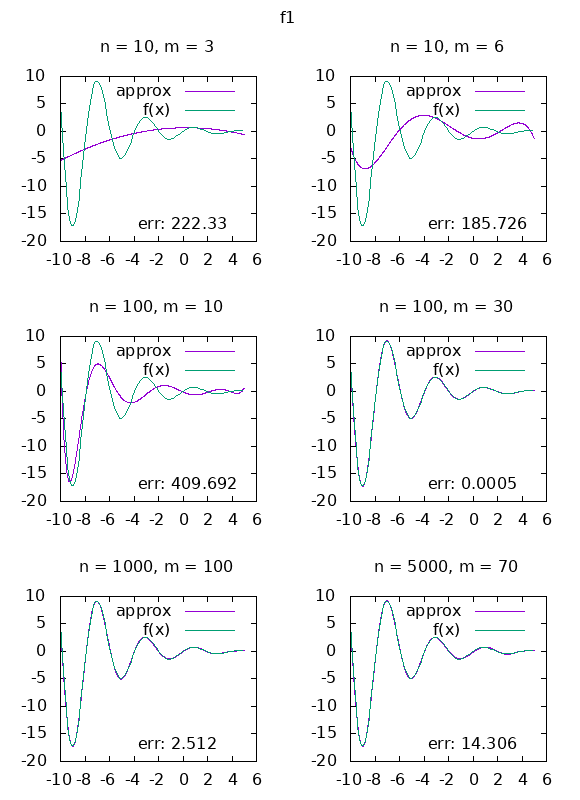
\includegraphics{graphs/plot1.png}

\clearpage
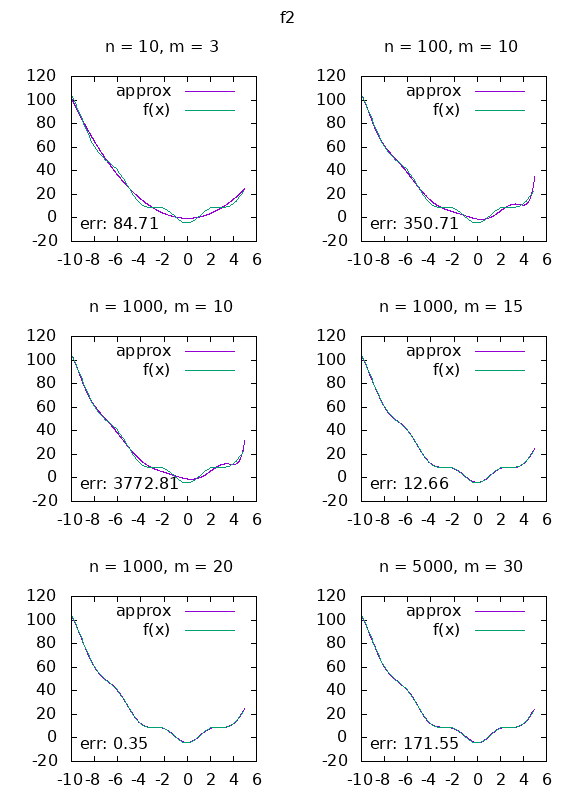
\includegraphics{graphs/plot2.png}

\clearpage
\section{Aproksymacja średniokwadratowa trygonometryczna}

\subsection{Funkcje testowe}

\[f_1(x) = exp(2cos(2x))\]
\begin{lstlisting}[language=C++]
func f1 = [](double x) { return exp(2 * cos(2 * x)); };
\end{lstlisting}

\[f_2(x) = sin(3x)exp(cos(2x))\]
\begin{lstlisting}[language=C++]
func f2 = [](double x) { return sin(3 * x) * exp(cos(2 * x)); };
\end{lstlisting}

\subsection{Opracowanie}

Za pomocą aproksymacji średniokwadratowej trygonometryczej możemy przybliżać funkcje okresowe o okresie \(2\pi\). Szukamy wielomianu trygonometrycznego postaci:
\[Q_n(x)={{a_0}\over{2}}+\sum_{k=1}^n(a_k\cos kx+b_k\sin kx)\]
gdzie \(n < L\). Punkty aproksymacji są postaci:
\[x_i={{\pi i}\over{L}}\mbox{ dla }i=0,1,2,..,2L-1\]
Korzystamy z metody średniokwadratowej, więc funkcja błędu wygląda następująco:
\[H=\sum_{i=0}^{2L-1}\left[f(x_i)-Q_n(x_i)\right]^2\]
Funkcja \(H\) przyjmuje wartość minimalną gdy parametry \(a_k\) i \(b_k\) są postaci:
\[a_k={{1}\over{L}}\sum_{i=0}^{2L-1}f(x_i)\cos k x_i={{1}\over{L}}\sum_{i=0}^{2L-1}f(x_i)\cos\left({{\pi ki}\over{L}}\right)\]
\[b_k={{1}\over{L}}\sum_{i=0}^{2L-1}f(x_i)\sin kx_i={{1}\over{L}}\sum_{i=0}^{2L-1}f(x_i)\sin\left({{\pi ki}\over{L}}\right)\]

\clearpage

\begin{lstlisting}[language=C++]
typedef std::pair<std::vector<double>, std::vector<double>> params;

params polynominal_params(int n, int L, func f) {
    params params;
    params.first = std::vector<double>();
    params.second = std::vector<double>();

    for (int j = 0; j < n; j++) {
        double sa = 0, sb = 0;

        for (int i = 0; i < 2 * L; i++) {
            double x = M_PI * i / L;
            sa += f(x) * cos(x * j);
        }

        for (int i = 0; i < 2 * L; i++) {
            double x = M_PI * i / L;
            sb += f(x) * sin(x * j);
        }

        params.first.push_back(sa / L);
        params.second.push_back(sb / L);
    }

    return params;
}
\end{lstlisting}

\begin{lstlisting}[language=C++]
double trig_polynomial(int n, params params, double x) {
    double s = 0.5 * params.first[0];
    for (int j = 1; j < n; j++) {
        s += params.first[j] * cos(j * x) + params.second[j] * sin(j * x);
    }

    return s;
}

double err(int n, int L, params params, func f) {
    double s = 0;
    for (int i = 0; i < 2 * L; i++) {
        double x = M_PI * i / L;
        s += pow(f(x) - tryg_polynomial(n, params, x), 2);
    }
    return s;
}
\end{lstlisting}
Funkcja \emph{polynominal\_params} oblicza wartości parametrów \(a_k\) i \(b_k\), natomiast funkcja \emph{trig\_polynomial} oblicza wartość wielomianu trygonometrycznego w danym punkcie. \emph{err} oblicza błąd średniokwadratowy.

\clearpage

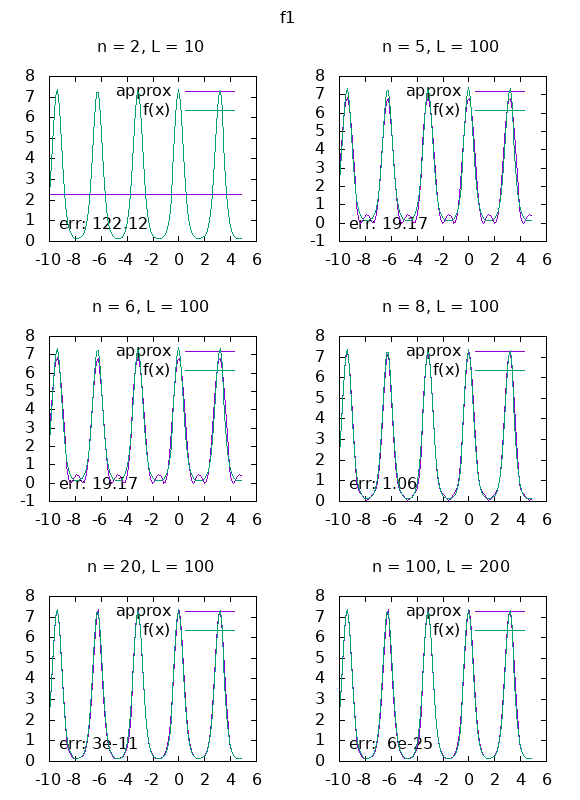
\includegraphics{graphs/plot3.png}

\clearpage
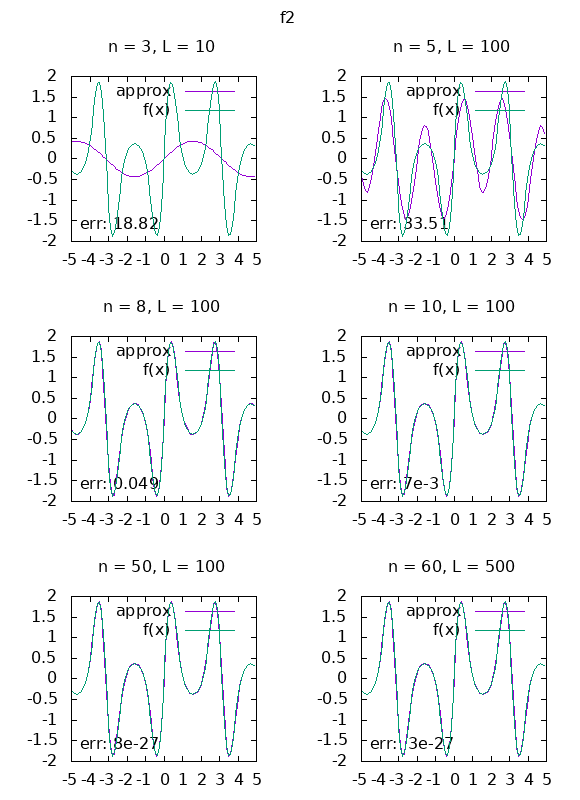
\includegraphics{graphs/plot4.png}
 
\end{document}
